\setchapterpreamble[u]{\margintoc}
\chapter{两因素被试间实验设计}
\labch{options}

%------------------------------------两因素完全随机实验设计
%\section{两因素完全随机设计}

\subsection{基本特点}
我在考查两种不同的教学方法对学生的影响时,发现它对学生的影响不显著,可我对这种教学方法还挺有自信的,于是我去调查了其原因.结果发现,学生的智力有不同,对于那些智力不太高的学生,他们接受新事物的能力不太高,在我换用新的教学方法后,他们的成绩反而下降.于是下接下的实验我同时考查这两个因素,结果发现教学方法的主效应还是不显著,不过学生的智力主效应倒是显著了,并且交互作用显著.这说明不同的教学方法适合不同的学生.

多因素实验设计的好处在上例中可以充分体现,自变量对因变量的关系有时因为别的变量的影响而被掩盖了,所以想要揭示变量间的真实关系需要做同时纳入多个变量.

最简单的因素实验设计是完全随机因素设计.一个两因素完全随机实验设计适合用于这样的研究条件:

(1)研究中有两个自变量,每个自变量有两个或多水平
(2)如果一个自变量有$p$个水平,另一个自变量有$q$个水平,实验中含有$p \times q$个处理的结合,研究者感兴趣于所有处理水平的结合的效应.

这种实验设计的基本方法是,随机分配被试接受实验处理的结合,每个被试接受一个实验处理的结合.与单因素完全随机设计不同,在两因素完全随机设计中,每个被试接受的是一个处理的结合,而不是一个处理水平.

\begin{margintable}
    \centering
    \caption{两因素完全随机被试分配到处理}
    \labtab{two_random_sub_teat}
    \begin{tabular}{cccccc}
    \toprule
        $a_1$ & $a_1$ & $a_1$ & $a_2$ & $a_2$ & $a_2$ \\
    \midrule
        $b_1$ & $b_2$ & $b_3$ & $b_1$ & $b_2$ & $b_3$ \\
        $S_1$ & $S_2$ & $S_3$ & $S_4$ & $S_5$ & $S_6$ \\
        $S_7$ & $S_8$ & $S_9$ & $S_{10}$ & $S_{11}$ & $S_{12}$ \\
        $S_{13}$ & $S_{14}$ & $S_{15}$ & $S_{16}$ & $S_{17}$ & $S_{18}$ \\
        $S_{19}$ & $S_{20}$ & $S_{21}$ & $S_{22}$ & $S_{23}$ & $S_{24}$ \\
    \bottomrule    
    \end{tabular}
\end{margintable}

两因素完全随机设计被试分配到处理上的情况如\reftab{two_random_sub_treat}

\subsubsection{两因素完全随机实验设计模型}

\begin{definition}[两因素完全随机实验设计模型]
    \labdef{two_way_random_model}
    \begin{align*}
        Y_{ijk} & = \mu + \alpha _j + \beta _k  + \left( \alpha \beta \right) _{jk}  + \varepsilon _{i\left( jk \right)}\\
                  & \left( j=1,2,\cdots ,p;  k=1,2,\cdots ,q;  i=1,2,\cdots ,n \right)
    \end{align*}
    
    其中
    
    {
        \renewcommand\arraystretch{1.25}
        \begin{tabular}{ccl}
            $Y_{ijk}$            & - &    两个自变量在第$j,k$个水平上,被试$i$的分数\\ 
            $\mu$                & - &    总体平均值或真值\\
            $\alpha _j$          & - &    自变量$A$水平$j$的处理效应\\
            $\pi _i$             & - &    自变量$B$水平$k$的处理效应\\
            $\left( \alpha \beta \right)_{jk}$ &-& 水平$\alpha _j$和$\beta _k$的交互作用\\
            $\varepsilon _i{jk}$  & - &   被试的误差变异
        \end{tabular}
    }  

\end{definition}

\subsubsection{两因素完全随机实验设计检验的假说}
(1)$A$因素的处理效应为0,即
\[ \alpha _j =0 \]

或$A$因素各水平总体均数相等,即
\[ \mu _{.1.} = \mu _{.2.} = \cdots = \mu _{.p.} \]


(2)$B$因素的处理效应为0,即
\[ \beta _k = 0 \]

或$B$因素各水平总体平均数相等,即
\[ \mu _{..1} = \mu _{..2} = \cdots = \mu _{..1} \]

(3)$AB$的交互作用为0,即
\[ \left( \alpha \beta \right) _{jk} = 0 \]


\subsection{实验设计与计算举例}
\subsubsection{研究的问题}

\textbf{1.计算表}

\begin{margintable}
  \centering
  \caption{两因素完全随机设计$ABS$表}
  \label{two_random_ABS}
    \begin{tabular}{cccccc}
    \toprule
        $a_1$ & $a_1$ & $a_1$ & $a_2$ & $a_2$ & $a_2$ \\
        $b_1$ & $b_2$ & $b_3$ & $b_1$ & $b_2$ & $b_3$ \\
    \midrule
        \rowcolor[rgb]{ .867,  .922,  .969} 3     & 4     & 5     & 4     & 8     & 12 \\
        \rowcolor[rgb]{ .867,  .922,  .969} 6     & 6     & 7     & 5     & 9     & 13 \\
        \rowcolor[rgb]{ .867,  .922,  .969} 4     & 4     & 5     & 3     & 8     & 12 \\
        \rowcolor[rgb]{ .867,  .922,  .969} 3     & 2     & 2     & 3     & 7     & 11 \\
    \bottomrule
    \end{tabular}
\end{margintable}

\begin{margintable}
  \centering
  \caption{两因素完全随机设计$AB$表}
  \label{two_random_AB}
    \begin{tabular}{c|cc|c}
    \toprule
          & $a_1$ & $a_2$ & $\sum$ \\
    \midrule
          & $n=4$ &       &  \\
    $b_1$ & \cellcolor[rgb]{ 1,  .949,  .8}16 & \cellcolor[rgb]{ 1,  .949,  .8}15 & \cellcolor[rgb]{ .886,  .937,  .855}31 \\
    $b_2$ & \cellcolor[rgb]{ 1,  .949,  .8}16 & \cellcolor[rgb]{ 1,  .949,  .8}32 & \cellcolor[rgb]{ .886,  .937,  .855}48 \\
    $b_3$ & \cellcolor[rgb]{ 1,  .949,  .8}19 & \cellcolor[rgb]{ 1,  .949,  .8}48 & \cellcolor[rgb]{ .886,  .937,  .855}67 \\
    \midrule
    $\sum$ & \cellcolor[rgb]{ .929,  .929,  .929}51 & \cellcolor[rgb]{ .929,  .929,  .929}95 & \cellcolor[rgb]{ .851,  .882,  .949}146 \\
    \bottomrule
    \end{tabular}
\end{margintable}


\textbf{2.各种基本量的计算}
\begin{alignat*}{4}
    &\frac{\left( \sum_{k=1}^q{\sum_{j=1}^p{\sum_{i=1}^n{Y_{ijk}}}} \right) ^2}{npq}
    &&=\left[ Y \right] 
    &&=\frac{\left( 146 \right) ^2}{\left( 4 \right) \left( 2 \right) \left( 3 \right)}
    &&= 888.167\\
    %---------------------------------------------------------------------------------------------------
    &\sum_{k=1}^q{\sum_{j=1}^p{\sum_{i=1}^n{Y_{ijk}^{2}}}}
    &&=\left[ ABS \right] 
    &&=\left( 3 \right) ^2+\left( 6 \right) ^2+\cdots 
    &&=1140.000\\
    %---------------------------------------------------------------------------------------------------
    &\sum_{j=1}^p{\frac{\left( \sum_{k=1}^q{\sum_{i=1}^n{Y_{ijk}}} \right) ^2}{nq}}
    &&=\left[ A \right] 
    &&=\frac{\left( 51 \right) ^2}{\left( 4 \right) \left( 3 \right)}+\frac{\left( 95 \right) ^2}{\left( 4 \right) \left( 3 \right)}
    &&=968.833\\
     %---------------------------------------------------------------------------------------------------
    &\sum_{k=1}^q{\frac{\left( \sum_{j=1}^p{\sum_{i=1}^n{Y_{ijk}}} \right) ^2}{np}}
    &&=\left[ B \right] 
    &&=\frac{\left( 31 \right) ^2}{\left( 4 \right) \left( 2 \right)}+\frac{\left( 48 \right) ^2}{\left( 4 \right) \left( 2 \right)}+\frac{\left( 67 \right) ^2}{\left( 4 \right) \left( 2 \right)}
    &&=969.250\\
    %---------------------------------------------------------------------------------------------------
    &\sum_{k=1}^q{\sum_{j=1}^p{\frac{\left( \sum_{i=1}^n{Y_{ijk}} \right) ^2}{n}}}
    &&=\left[ AB \right] 
    &&=\frac{\left( 16 \right) ^2}{4}+\frac{\left( 15 \right) ^2}{4}+\cdots 
    &&=1106.500
\end{alignat*}


\textbf{3.平方和分解与计算}

\begin{definition}[两因素完全随机平方和分解]
\labdef{two_way_random_variance}
\begin{alignat*}{3}
    &    SS_{\text{总变异}}     &&=    SS_{\text{处理间}}    &&+    SS_{\text{处理内}}\\
    &                           &&=    \left( SSA + SSB + SSAB \right) &&+ SS_{\text{单元内}}
\end{alignat*}
\end{definition}

\begin{alignat*}{3}
    &    SS_{\text{总变异}}    &&=    [ABS] - [Y]                              &&=    251.833\\
    &    SSA                   &&=    [A]   - [Y]                              &&=    80.666\\
    &    SSB                   &&=    [B] - [Y]                                &&=     81.083\\
    &    SSAB                  &&=    [AB] - [Y] - SSA - SSB                   &&=    56.584\\
    &    SS_{\text{单元内}}    &&=     SS_{\text{总变异}} - SSA -SSB - SSAB     &&= 33.500
\end{alignat*}

\textbf{4.方差分析表及结果的解释}


\begin{table}[htbp]
	\centering
	\caption{两因素完全随机方差分析表}
	\labtab{two_way_random_ANOVA}
	{
		\begin{tabular}{lrrrrrr}
			\toprule
			\multicolumn{1}{c}{变异源} & \multicolumn{1}{c}{$SS$} & \multicolumn{1}{c}{$df$} & \multicolumn{1}{c}{$MS$} & \multicolumn{1}{c}{$F$} & \multicolumn{1}{c}{$p$} \\
			\midrule
			$A$(主题熟悉性) & 80.667 & 1.000 & 80.667 & 43.343 & $<$ .001  \\
			$B$(生字密度) & 81.083 & 2.000 & 40.542 & 21.784 & $<$ .001  \\
			$A \times B$ & 56.583 & 2.000 & 28.292 & 15.201 & $<$ .001  \\
			单元内误差 & 33.500 & 18.000 & 1.861 &  &    \\
			\bottomrule
		\end{tabular}
	}
\end{table}


\textbf{5.平方和与自由度分解图}

\subsection{一些解释}
\textbf{1.各种平方和的意义}

\textbf{2.同质性检查}
\begin{alignat*}{3}
    & SS_{\text{1组}} &&= \left( 3^2+6^2+\cdots \right) -\frac{\left( 16 \right) ^2}{4}    &&=    6\\
    & SS_{\text{2组}} &&= \left( 4^2+6^2+\cdots \right) -\frac{\left( 16 \right) ^2}{4}    &&=    8\\
    & SS_{\text{3组}} &&= \left( 5^2+7^2+\cdots \right) -\frac{\left( 19 \right) ^2}{4}    &&=    12.75\\
    & SS_{\text{4组}} &&= \left( 4^2+5^2+\cdots \right) -\frac{\left( 15 \right) ^2}{4}    &&=    2.75\\
    & SS_{\text{5组}} &&= \left( 8^2+9^2+\cdots \right) -\frac{\left( 32 \right) ^2}{4}    &&=    2\\
    & SS_{\text{6组}} &&= \left( 12^2+13^2+\cdots \right) -\frac{\left( 48 \right) ^2}{4}  &&=    2\\
    & F               &&=\frac{SS_{\text{最大}}}{SS_{\text{最小}}}=\frac{12.75}{2}         &&=6.375
\end{alignat*}

计算$F(3,3)=6,375$对应的概率,得到$p>.05$,表明6组被试是同质的.如果把上述6个组的平方和相加,可以得到直接计算单元内误差,这和前面用相减法得到的结果相同.
\[ SS_{\text{单元内}} = SS_{\text{1组}}+SS_{\text{2组}}+\cdots+SS_{\text{6组}}=33.500 \]
%------------------------------------两因素交互作用的探讨
%\input{chapters/two_between/cross.tex}

\section{两因素交互作用的进一步探讨}

\subsection{交互作用含义}

前面我用教学方法和智力的例子大体说明了这个问题,教学方法对阅读成绩的成绩不仅与其本身是新教学方法还是旧教学方法有关,也受到学生智力的影响.换句话说,高智力学生可以接受到新教学方法的好处,相反低智力学生不仅不能体会其好处,而且可能因为他们不适应新的教学方法导致成绩不增反降.因此我们得到交互作用的定义:

\begin{definition}[交互作用]
\labdef{cross_effect}
    指的是一个因素的的效应在一个或多个因素不同的水平上不同.
\end{definition}

\vreffig{two_cross}展示了两因素交互作用可能存在8种情况,我将单因素时得到的结果用蓝色线段加粗标出来,可以看到,$A$因素主效应不显著会对应(1)~(4)四种情况,而只有(1)和(2)是真的可以说明因素$A$对因变量没有影响;(3)和(4)这种情况下,$A$因素的效应在$B$因素的两个水平下是相反的,而且总体上恰好抵消了,显得好像$A$因素对因变量没有效应似的,在多因素解释效应时要小心.

在交互作用显著的(3)(4)(7)(8)中,(3)(4)(7)表示的交互作用中两条线段交叉,表明$A$的效应在不同$B$的水平上相反,称为\textbf{非同序交互作用(disordinal interaction)}
\marginnote{\textbf{非同序交互作用(disordinal interaction}指的是在因素$B$不同组上,因素$A$的效应方向相反}.
(8)表示的交互作用中,$B$不同组中$A$的效应还是一个方向的,称之为\textbf{同序交互作用(ordinal interaction)}.
\marginnote[*2]{\textbf{同序交互作用(ordinal interaction)}指的是在因素$B$不同组上,因素$A$的效应方向相同}

\begin{figure*}
    \includegraphics{cross}
    \caption{两因素交互作用可能的8种情况,中间蓝色的加粗线为$A$因素的简单主效应,可以看到只考虑一种因素会掩盖很多信息。(1)和(5)中三条线本是重合的,但是为了可以看得清楚故将其稍微拉开了一点,(8)中绿色的虚线和实线表示$b_1$这两种状况都属于这种情况}
    \labfig{two_cross}
\end{figure*}

\subsection{交互作用图解}
当方差分析表明两个因素的交互作用是显著的时候,研究者常常需要进一步了解交互作用的含义是什么.一种简单的方法是画出交互作用的图解,以观察一个因素的各水平在另一个因素的每个水平上的变化.作图解时,应首先计算出每个处理水平结命中所得到的平均数,然后以平均数作图.我们仍举上面两因素完全随机设计的例子,列出它的$AB$表(\reftab{two_random_AB_2}和\reftab{two_random_AB_avg})

\begin{margintable}
  \centering
  \caption{两因素完全随机设计$ABS$表}
  \labtab{two_random_AB_2}
    \begin{tabular}{ccc}
    \toprule
          & $a_1$ & $a_2$ \\
    \midrule
          & $n=4$ &  \\
    $b_1$ & 16    & 15 \\
    $b_2$ & 16    & 32 \\
    $b_3$ & 19    & 48 \\
    \bottomrule
    \end{tabular}%
\end{margintable}

\begin{margintable}
  \centering
  \caption{两因素完全随机设计$AB$平均数表}
  \labtab{two_random_AB_avg}
    \begin{tabular}{ccc}
        \toprule
              & $a_1$ & $a_2$ \\
        \midrule
        $b_1$ & 4     & 3.75 \\
        $b_2$ & 4     & 8 \\
        $b_3$ & 4.75  & 12 \\
        \bottomrule
    \end{tabular}
\end{margintable}

根据$AB$平均数表,可双两个方向作用(\reffig{AB_cross_two_directions})

\begin{figure}
    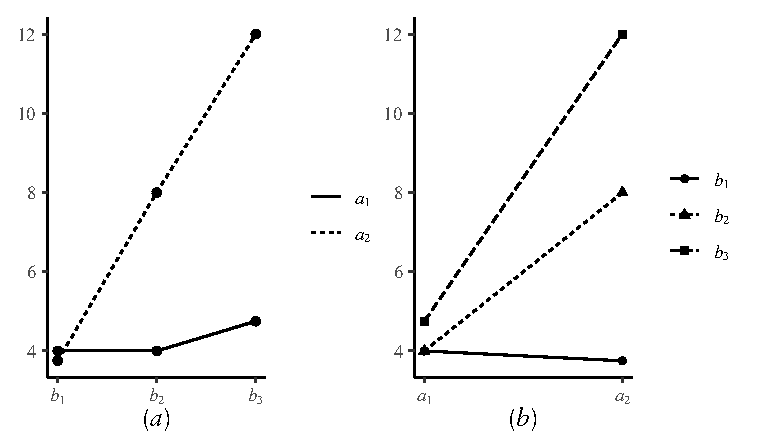
\includegraphics{cross_effect_two_directions}
    \caption{$AB$交互作用两个方向的图}
    \labfig{AB_cross_two_directions}
\end{figure}



对两个图的解释是不一样的,\reffig{AB_cross_two_directions}(a)表明,$B$因素在$A$因素的两个水平上影响趋势是不一致的.$B$因素的三个水平在$a_1$水平似乎没有明显差别,而在$a_2$水平有较大差异.
\reffig{AB_cross_two_directions}(b)表明,$A$因素在$B$因素的三个水平上的影响趋势也不一致.$A$因素的两个水平在$b_1$水平没有明显差异,而在$b_2,b_3$水平存在较大差异.

图解法的优点是简单、直观.直接利用各处理水平结合所得的平均观测值作图,可以使读者对结果模式有一个非常直观的了解.它的弱点是,解释是主观的,有时不同的研究者可能会对同一结果作出不同的解释,尤其是当出现复杂的交互作用时,研究者单靠经验、直观进行解释是很困难的.因此,图解一般只能作为检查交互作用的第一步,它需要同统计检验结合起来,以便进一步用数据对交互作用的意义作出更精确可靠的解释.

\subsection{简单效应检验}
\subsubsection{基本特点}

检查交互作用含义的另一个方法是简单效应检验,简单效应检验与主效应检验不大相同.主效应检验是在忽略其它因素的情况下检验一个因素的处理效应,我们比较一下主效应和简单效应的不同之处.

设观测值为$Y_{ijk}$,$i$是处理组合内的第$i$个被试,$j$是因素$A$的的水平$j$,$k$是因素$B$的水平$k$

1. $A$因素和$B$因素的\textbf{主效应}用组内平均数与真值的差估计,组内平均数忽略了被试和其它因素,可表示为
\[ \begin{array}{cc}
    \alpha _1 = \mu _{.1.} - \mu    &    \beta _1 = \mu _{..1} - \mu\\ 
    \alpha _2 = \mu _{.2.} - \mu    &    \beta _2 = \mu _{..2} - \mu\\
    \vdots                          &     \vdots \\
    \alpha _j = \mu _{.j.} - \mu    &    \beta _k = \mu _{..k} - \mu\\
    
    \alpha _p = \mu _{.p.} - \mu    &    \beta _q = \mu _{..q} - \mu
\end{array}\]

可检验的假说是:

(1)$A$因素处理水平上的总体平均数相等,即:
\[H_0 : \mu _{.1.} = \mu _{.2.} = \cdots = \mu _{.p.}\]

或$A$因素处理效应为0,即:
\[ \alpha _j = 0 \]

(2)$B$因素处理水平上的总体平均数相等,即:
\[ H_0 : \mu _{..1} = \mu _{..2} = \cdots = \mu _{..q} \]

或$B$因素处理效应为0,即:
\[ \beta _k =0 \]

2.\textbf{简单效应}

%这段话没写好

本例中,对于因素$A$,我们分别计算它的效应在$b_1,b_2,b_3$上的变异,
\reffig{AB_cross_two_directions}(b)上三条线段因为斜率不一样所以我们怀疑可能存在交互作用,而上述拆分的三个变异的显著性正好反应这条线在统计上是显著的平还是显著的斜
如果$A$在$b1$上的变异不显著,而在$b_2,b_3$上的变异显著,则说明确实存在交互作用.

所以说简单效应的计算也就是将一个因素对因变量的效应拆分成多组,有另一个因素有多少水平就拆分成多少个组,我们检验它在另一个因素不同水平上的显著性.

\[\begin{array}{cc}
    \alpha _{1\left( \text{在}b_1\text{水平上} \right)} = \mu _{.11} - \mu _{..1} & \beta _{1\left( \text{在}a_1\text{水平上} \right)} = \mu _{.11} - \mu _{.1.}\\
    \alpha _{2\left( \text{在}b_1\text{水平上} \right)} = \mu _{.21} - \mu _{..1}& \beta _{2\left( \text{在}a_1\text{水平上} \right)} = \mu _{.12} - \mu _{.2.}\\
    \vdots                                              & \vdots\\
    \alpha _{j\left( \text{在}b_1\text{水平上} \right)} = \mu _{.j1} - \mu _{..1}&\beta _{k\left( \text{在}a_1\text{水平上} \right)}= \mu _{.1k} - \mu _{.1.}\\
    \vdots                                              & \vdots\\
    \alpha _{j\left( \text{在}b_k\text{水平上} \right)} = \mu _{.jk} - \mu _{..k}& \beta _{k\left( \text{在}a_j\text{水平上} \right)}= \mu _{.jk} - \mu _{j.}\\
    \vdots                                              & \vdots\\
    \alpha _{p\left( \text{在}b_q\text{水平上} \right)} = \mu _{.pq} - \mu _{..q}& \beta _{q\left( \text{在}a_p\text{水平上} \right)}= \mu _{.pq} - \mu _{.p.}
\end{array}\]




\subsubsection{计算举例}

\begin{table}[htbp]
	\centering
	\caption{两因素完全随机方差分析与两个方向简单效应检验}
	\labtab{two_random_simple_mail_effect}
	{
                    \begin{tabular}{lrrrrrr}
		    \toprule
			\multicolumn{1}{c}{变异源} & \multicolumn{1}{c}{$SS$} & \multicolumn{1}{c}{$df$} & \multicolumn{1}{c}{$MS$} & \multicolumn{1}{c}{$F$} & \multicolumn{1}{c}{$p$} \\
			\midrule
			$A$ & 80.667 & $p-1=1$ & 80.667 & 43.343 & $<$ .001  \\
			$B$ & 81.083 & $q-1=2$ & 40.542 & 21.784 & $<$ .001  \\
			$A\times B$ & 56.583 & $(p-1)(q-1)=2$ & 28.292 & 15.201 & $<$ .001  \\
		    \midrule
			$A_{\left( \text{在}b_1\text{水平} \right)}$ & 0.125 & $p-1=1$ & 0.125 & 0.067 & 0.798  \\
			$A_{\left( \text{在}b_2\text{水平} \right)}$ & 32.000 & $p-1=1$ & 32.000 & 17.194 & $<$ .001  \\
			$A_{\left( \text{在}b_3\text{水平} \right)}$ & 105.125 & $p-1=1$ & 105.125 & 56.485 & $<$ .001  \\
		    \midrule
			$B_{\left( \text{在}a_1\text{水平} \right)}$ & 1.500 & $q-1=2$ & 0.750 & 0.403 & 0.674  \\
			$B_{\left( \text{在}a_2\text{水平} \right)}$ & 136.167 & $q-1=2$ & 68.083 & 36.582 & $<$ .001  \\
		    \midrule
		        单元内误差 & 33.500 & $pq(n-1)=18$ & 1.861\\
		    \bottomrule
		\end{tabular}
	}
\end{table}

\subsubsection{使用}
%------------------------------------两因素随机区组实验设计
\section{两因素随机机区组实验设计}


\begin{tikzpicture}[node distance=30mm,
  every node/.style = {shape=rectangle, 
    draw, align=center,}]]
  \node {$SS_{\text{总变异}}$\\$df=npq-1$}
    child{ node {$SS_{\text{处理间}}$\\$df=pq-1$} 
            child { node{$SSA$\\$df=p-1$}}
            child {node{$SSB$\\$df=q-1$}}
            child {node{$SSAB$\\$df=(p-1)(q-1)$}}        
    }  
    child 
    { 
        node{$SS_{\text{处理内}}$ \\ $df=pq(n-1)$}
        child{
            node{$SS_{\text{单元内}}$\\$df=pq(n-1)$} 
        }        
    };
\end{tikzpicture}
